%!TEX root = ../../super_main.tex
\section{Structural Sensor Data}
\label{sec:structural_sensor_data}

% Det bliver hurtigt til meget data når man arbejder med continious data
% Vi bruger sample frequency til at lave mellemrum mellem samples i tid fordi det ikke er så brugbart at have 8gb data for et minuts målinger
% Vi vil gerne have flere measurements per sample så vi kan undgå upræcise målinger

We have come up with a solution to the concerns described in \secref{sub:data_quantity_estimation}. We have decided to facilitate periodic data collection instead of continuous readings of data in order to facilitate different data needs. \figref{fig:sample_temporality} illustrates how samples are collected. A sample consists of multiple measurements to allow for further precision. Both sample frequency and measurement frequency are configurable.

\todo[inline]{Vi har reelt 3 forskellige tider: Hvor længe skal et sample vare, hvor ofte skal vi tage et sample, hvor længe skal der gå imellem measurements i et sample? På grund af at sensore i Android giver svar når de har lyst, er det ikke sikkert at der kommer den samme mængde measurements i hver sample. Vi skal overveje om det giver mening, eller om det er vigtigere for kunden at hvert sample med garenti indeholder x measures. Problemet med dette er så at vi ikke kan sætte nogen garenti for hvornår disse measures reelt kommer.} 

\begin{figure}[!htbp]
    \centering
    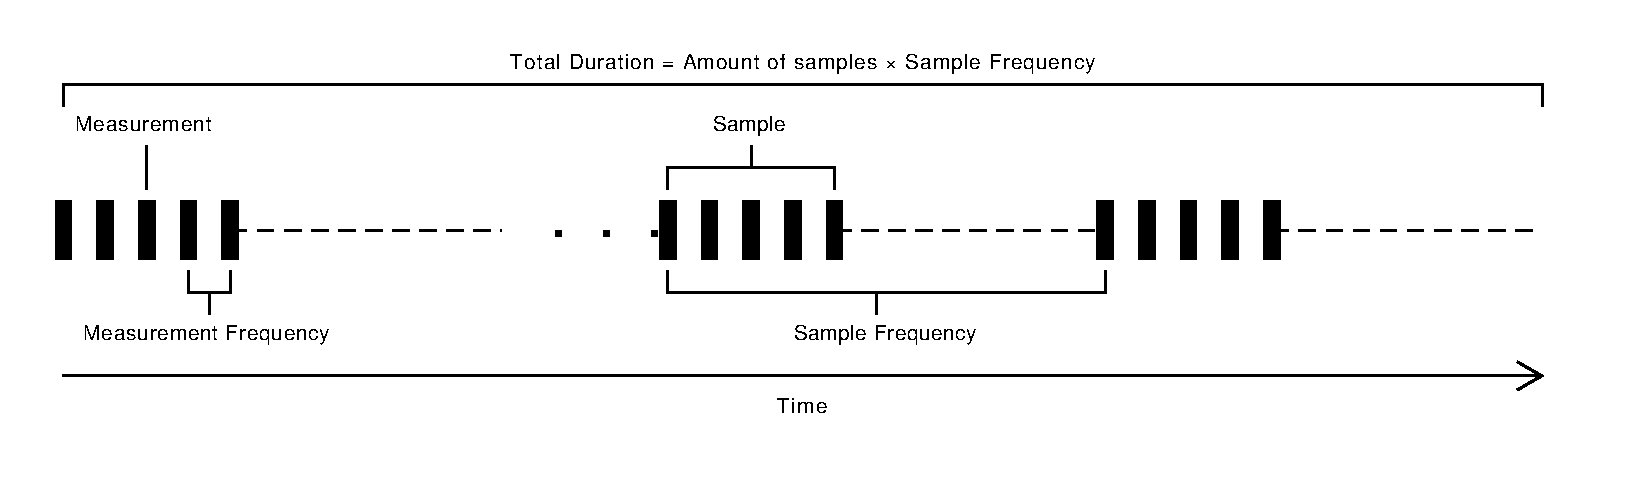
\includegraphics[width=\textwidth]{unsorted/sample_temporality}
    \caption{Overview of sample and measurement temporality.}
    \label{fig:sample_temporality}
\end{figure}
\FloatBarrier